
%     %%%%%%%%%%%%%%%
%
%     P A C K A G E S
%
%     %%%%%%%%%%%%%%%

\documentclass[11pt, a4paper]{article}
\usepackage{fontspec}
\usepackage{caption}
\usepackage{mathtools}
\usepackage{gensymb}
\usepackage{float}

% DOCUMENT LAYOUT
\usepackage{geometry}
\geometry{a4paper, textwidth=42em, textheight=70em, marginparsep=0.5em, marginparwidth=3.5em}
\setlength\parindent{0em}
\setlength\parskip{0.75em}
\captionsetup{width=0.8\textwidth}

% FONTS
\usepackage[usenames,dvipsnames]{xcolor}
\usepackage{xunicode}
\usepackage{xltxtra}
\defaultfontfeatures{Mapping=tex-text}
%\setromanfont [Ligatures={Common}, Numbers={OldStyle}, Variant=01]{Linux Libertine O}
%\setmonofont[Scale=0.8]{Monaco}
%%% modified by Karol Kozioł for ShareLaTeX use
\setmainfont[
  Ligatures={Common}, Numbers={OldStyle}, Variant=01,
  BoldFont=LinLibertine_RB.otf,
  ItalicFont=LinLibertine_RI.otf,
  BoldItalicFont=LinLibertine_RBI.otf
]{LinLibertine_R.otf}
\setmonofont[Scale=0.8]{DejaVuSansMono.ttf}

% HEADINGS
\usepackage{sectsty}
\usepackage[normalem]{ulem}
\sectionfont{\mdseries\upshape\Large}
\subsectionfont{\mdseries\scshape\normalsize}
\subsubsectionfont{\mdseries\upshape\normalsize}

\renewenvironment{abstract}{%
{\mdseries\scshape\Large\abstractname}
\vspace{1em}\\
}{\par\noindent}


\usepackage[superscript]{cite}

% LISTINGS
\usepackage{listings}
\usepackage{color}
\usepackage{appendix}

\usepackage{color}
\definecolor{codered}{rgb}{0.61,0.21,0.18}
\definecolor{codegreen}{rgb}{0,0.6,0}
\definecolor{codegray}{rgb}{0.5,0.5,0.5}
\definecolor{codepurple}{rgb}{0.58,0,0.82}
\definecolor{backcolour}{rgb}{1.0,1.0,1.0}
\lstset{
  backgroundcolor=\color{backcolour},   
  commentstyle=\color{codegray},
  keywordstyle=\color{codered},
  numberstyle=\tiny\color{codegreen},
  stringstyle=\color{codepurple},
  basicstyle=\footnotesize\ttfamily,        % the size of the fonts that are used for the code
  breaklines=true,                          % sets automatic line breaking
  keepspaces=true,                          % keeps spaces in text, useful for keeping indentation of code
  showspaces=false,                         % show spaces everywhere adding particular underscores; it overrides 'showstringspaces'
  showstringspaces=false,                   % underline spaces within strings only
  showtabs=false,                           % show tabs within strings adding particular underscores
  stepnumber=2,                             % the step between two line-numbers. If it's 1, each line will be numbered
  tabsize=4, 	                            % sets default tabsize to 2 spaces
  title=\lstname                            % show the filename of files included with \lstinputlisting
}


%     %%%%%%%%%%%%%%%
%
%     D O C U M E N T
%
%     %%%%%%%%%%%%%%%


\begin{document}
\title{IAR Task 2 Report}
\author{Angus Pearson -- s1311631\\ Jevgenij Zubovskij -- s1346981}
\date{\today}
\maketitle

%       ^v^v^v^v^v^v^v^v^v^v^v^v^v^v^v^v^v^v^v^v^v^v^v^v^v^v^v^v^v^v^v^v^v^v^v^


\begin{abstract}
  We present an implementation of an algorithm similar to \textit{Bug2} \cite{principlesrobot} 
  built atop reactive obstacle collision avoidance and edge following behaviour developed for 
  \textit{Task1} with the \textit{Khepera} robot. The existing architecture is extended to
  include storing and publishing timestamped poses and goal state to a Redis \cite{Redis} server.
  Real-time visualisation using a Redis to ROS \cite{ROS} pipe provides a graphical display 
  of odometry, sensory information and goals in Rviz. After-the-fact plotting is provided 
  with MatPlotLib independent of ROS.

  In our testing, the robot was able to navigate to within 10cm of the origin (it's home location) 
  from any location in an environment successfully in 17/20 experiments, where each 
  environment was designed to evoke edge-case behaviour considered hard for the algorithm. The 
  algorithm performs similarly in both a static world and dynamic one in which other actors 
  (e.g. Humans) present a transient obstacle. 
\end{abstract}

%       ^v^v^v^v^v^v^v^v^v^v^v^v^v^v^v^v^v^v^v^v^v^v^v^v^v^v^v^v^v^v^v^v^v^v^v^


\section{Introduction}
\label{Introduction}

The second IAR assignment entails extending the existing systems from Task 1 with Odometry, 
to maintain an estimate of the robot's location. The task also calls for `return to home' ability, 
``either by retracing its outward route or more directly''. As an extension, basic mapping 
of the world is developed (without localisation correction for odometry dead-reckoning drift). 

This new return home behaviour is implemented as extension to the simpler reactive wall-following
and collision avoidance code from \textit{Task1}\cite{task1_report}, in a hybrid-subsumtive sense 
where the higher-level return navigation generally informs the Robot's behaviour, but if proximity
thresholds are violated the lower level reaction will peturb the trajectory away from an obstacle
until the proximity error clears.

We use Rviz for real-time plotting, a popular graphical tool for ROS to live-render the 
Robot's pose, odometry trail, obstacles perceived by the IR range sensors and goals. 
Rviz is plotting standard ROS messages such as Poses, Paths and Point Clouds that we publish 
to `ROS topics'.


%       ^v^v^v^v^v^v^v^v^v^v^v^v^v^v^v^v^v^v^v^v^v^v^v^v^v^v^v^v^v^v^v^v^v^v^v^

\newpage
\section{Odometry}
\label{Odometry}


We use odometry to find the Pose of the robot ${(x,y,\Theta)}$. The starting position of the robot as the origin of the coordinate system ${(0, 0)}$
and the forward-facing direction of the robot as the positive direction of the $x$ axis and
all angles are measured in relation to that. Ideally we would like to account for odometry drift
over time due to wheel slippage, encoder error and approximate calculations etc.

Moreover, we assume that the wheels have equal diameter and that the data given in the 
Khepera 2 User Manual \cite{khepera_manual} is correct and an increment of 12 encoder ticks 
means a wheel has advanced 1mm in it's rotational direction.

An advantage of the Khepera is that it has very thin wheels, meaning almost a single point of contact
to the floor, which make odometry much more accurate.

\subsection{Research}

Before settling on a method to use, we researched several papers and websites for inspiration or 
already fully conceptualized solutions or even a fully developed and tested approach. The first one
we found used a fourth order \textit{Runge-Kutta} numerical integrator \cite{runge_kutta} and looked like 
it would compensate for non-ideal encoders. However, upon implementation, and  testing if it correctly 
detects the robot going in a straight line (equal motor speeds) and said algorithm failing to significantly reduce error, it was abandoned. 

Hence, a simple yet mathematically sound approach \cite{odo_used} was adopted. 



\subsection{Chosen Method}

Pose calculation\cite{odo_used} uses simple trigonometry and differential drive on 
the wheels to perform its task. The position for 
${(x,y,\Theta)}$ are in the global reference pane, relative to initial position.

\begin{enumerate}

	\item Distance driven by each wheel 
          ${\Delta s_{wheel} = \frac {\Delta ticks_{wheel} } {12 ^{ticks}/_{mm}}}$
	\item Total distance driven ${\Delta s = \frac{\Delta s_{r} + \Delta s_{l} }{2}}$
	\item Change in heading ${\Delta\Theta = \frac{ \Delta s_{r} - \Delta s_{l} }{B}}$ 
          where $B$ is the wheel base (distance between points of contact of the two wheels on the floor)
	\item $x$ position update ${x_{n+1} = x_{n} + \Delta s \cos (\Theta_n + \frac{\Delta\Theta}{2})}$
	\item $y$ position update ${y_{n+1} = y_{n} + \Delta s \sin (\Theta_n + \frac{\Delta\Theta}{2})}$
        \item Lastly update ${\Theta_{n+1} = \Theta_{n} + \Delta\Theta}$


\end{enumerate}

The encoders are incremental and are able to detect both forward and backward movement 
of the wheel, so no software switching is required to differentiate forward and reverse
motion.

We do not use Odometry to inform navigation other than by the \textit{\S\ref{Return Algorithm}
 Return Algorithm} to ensure the robot is within the desired radius of the goal.

\subsection{Calibration}

The odometry was tested in a square box to verify it identifies $90$\degree turns correctly 
(while following the walls of the box) as well as representing accurate distance. We calibrated 
according to the methods laid out in \cite{odo_calibration}. We reduced the wheelbase if the 
angle was shown to be too small and increase if it was too large until  the odometry detected 
the  $90$\degree turns correctly. The actual $5$ cm wheelbase is calibrated to $5.6$ cm in code.

Figure \ref{rightanglecalib} shows a diagram of a simple test to ensure the actual right-angle 
turn is reflected correctly in odometry.

\begin{figure}[H]
  \begin{center}
    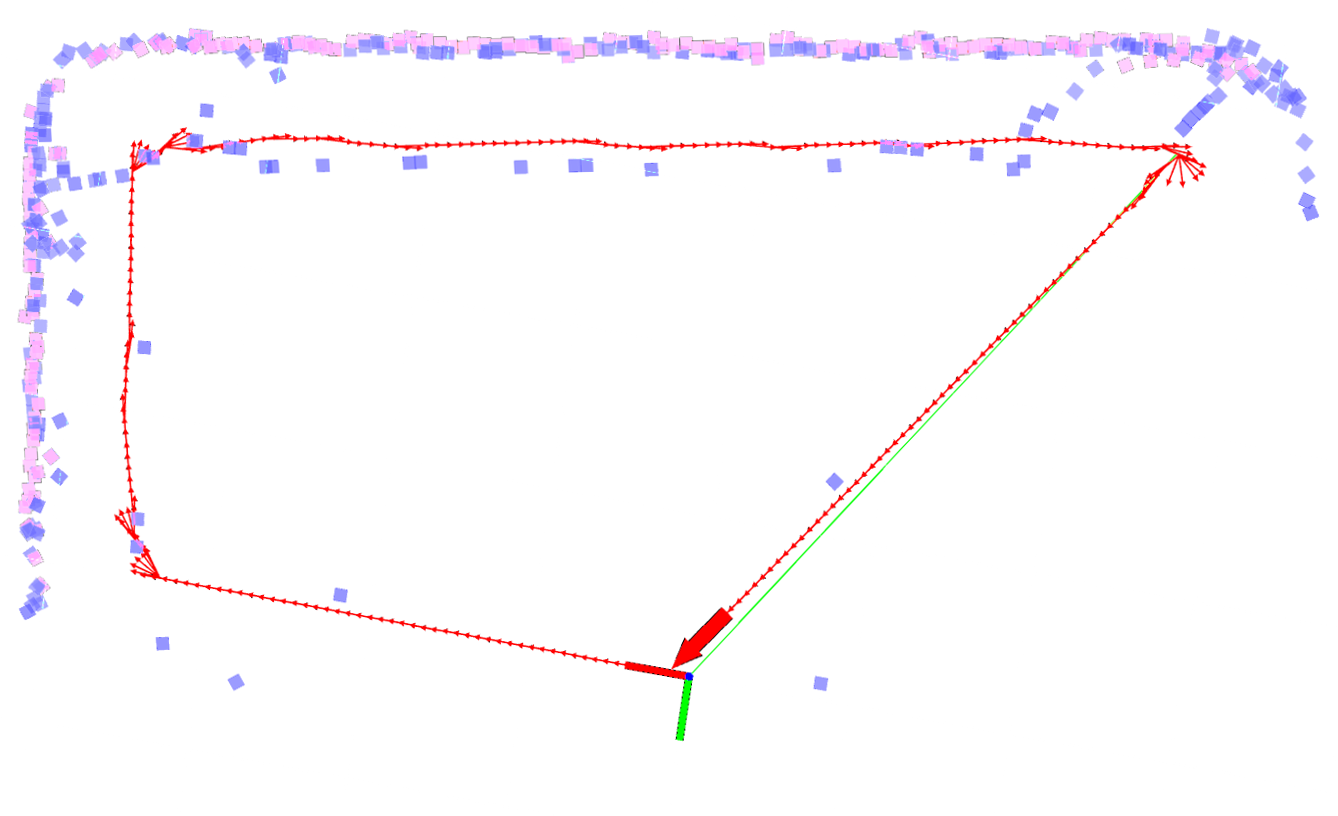
\includegraphics[width=30em]{../assets/right-angle-calibration.png}
    \caption{\label{rightanglecalib}The robot starts in the centre of an empty square box, heads towards the wall, turns to follow the wall, then turns the box corner which is $90$ \degree, follows the wall for some more time, and heads to its starting position (where it stops).}
  \end{center}
\end{figure} 




%       ^v^v^v^v^v^v^v^v^v^v^v^v^v^v^v^v^v^v^v^v^v^v^v^v^v^v^v^v^v^v^v^v^v^v^v^

\section{Return Algorithm}
\label{Return Algorithm}

Since Task 2 requires odometry, we localise solely with odometry and use the IR sensors for 
avoiding obstacles as per \textit{Task 1}\cite{task1_report}.

%       ^v^v^v^v^v^v^v^v^v^v^v^v^v^v^v^v^v^v^v^v^v^v^v^v^v^v^v^v^v^v^v^v^v^v^v^

\subsection{Research}

Choset's so-called \textit{Bug algorithms}\cite{principlesrobot}, inspired by insect behaviour
give simple behaviour capable of navigating to a location suitable for the task. \textit{Bug 2} is
robust and in most environments the most efficient out of the three Bug algorithms. 
Hence, it was chosen to be implemented.


%       ^v^v^v^v^v^v^v^v^v^v^v^v^v^v^v^v^v^v^v^v^v^v^v^v^v^v^v^v^v^v^v^v^v^v^v^


\subsection{Method Chosen}

The Bug 2 algorithms is conceptually simple. The assumptions it needs to work properly can 
be simplified to:

\begin{enumerate}

	\item Known direction to goal and robot can measure distance between points
	\item Be in a bounded workspace with a finite number of finite size objects

\end{enumerate}

These assumptions are satisfied by the environment for the task.

\begin{figure}[H]
  \textbf{\scshape Bug 2 Algorithm}
  
  \begin{enumerate}
    
  \item Head toward goal on the \textit{m-line} -- the straight line drawn from the start point to the goal
  \item If an obstacle is in the way, follow it until you encounter the \textit{m-line} again closer to the goal
  \item Leave the obstacle and continue toward the goal
    
  \end{enumerate}
\end{figure}

\begin{figure}[H]
  \begin{center}
    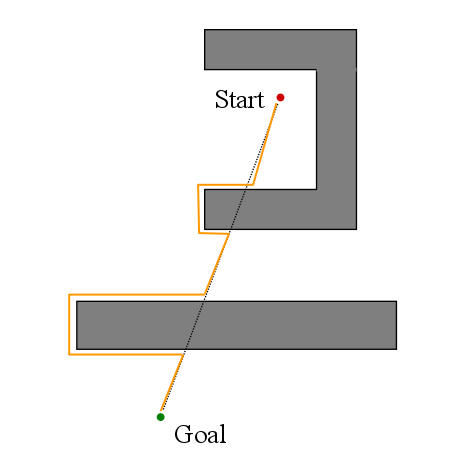
\includegraphics[width=20em]{../assets/bug-algorithm-diagram.png}
    \caption{Example Bug 2 operation diagram.
      The straight line between the Start and Goal is the \textit{m-line}}
  \end{center}
\end{figure}


%       ^v^v^v^v^v^v^v^v^v^v^v^v^v^v^v^v^v^v^v^v^v^v^v^v^v^v^v^v^v^v^v^v^v^v^v^

\subsection{Integration}

The algorithm is activated after $\approx 30$ seconds of exploration\cite{task1_report} and after
activation is the dominant algorithm unless one of the following is true for that control loop iteration:

\begin{enumerate}	

	\item The reactive control (getting unstuck \cite{task1_report}) activates - reactive avoidance algorithm is in control
	\item There is a miscalculation for the new speeds and they robot may try to drive towards the wall it is following - exploration (navigation) algorithm is in control

\end{enumerate}

The second point can occur if \textit{m-line} recomputation occurs as described in \textit{m-line Replanning}

Figure \ref{controlflow} shows how the controling paradigm is chosen from Reactive Avoidance, 
explorative Navigation and Return at every iteration of the loop. Before the 30 second mark robot
performs exactly as per \textit{Task 1}, after that the ``boredom''\cite{task1_report} is disabled. 
Please note that unlike in the report for \textit{Task 1}, here the collision avoidance is regarded
as a separate algorithm from the wall following, forward driving and ``boredom'' (exploration algorithm) one

The following is a representation of the algorithm in a state diagram form:
\begin{figure}[H]
  \begin{center}
    \includegraphics[width=30em]{../assets/control-choice-diagram.png}
    \caption{\label{controlflow}Control algorithm selection in a state diagram form.}
  \end{center}
\end{figure} 


%       ^v^v^v^v^v^v^v^v^v^v^v^v^v^v^v^v^v^v^v^v^v^v^v^v^v^v^v^v^v^v^v^v^v^v^v^

\subsection{Applied Alterations}
\label{Needed Alterations}

However, the implementation is much less trivial than the higher level description. It it had 
to be altered due to problems that became evident during testing and in \textit{\S\ref{Results} Experimental Results}

%       ^v^v^v^v^v^v^v^v^v^v^v^v^v^v^v^v^v^v^v^v^v^v^v^v^v^v^v^v^v^v^v^v^v^v^v^


\subsubsection{Thresholding}

Due to imperfect encoders, wheel slippage, odometry drift and being unable to sample odometry 
more often than every $20$ ms\cite{khepera_manual} (due to sequential 
reads of IR being in the same loop. Moreover, one must remember odometry fomulae have intrinsic 
systematic error.

Hence, all odometry and position-related calculations can not be strict equalities to compensate 
for the above error. Hence, all values are considered ``on-point'' as long as their value
fall within the expected range. Some thresholds are several centimetres.


%       ^v^v^v^v^v^v^v^v^v^v^v^v^v^v^v^v^v^v^v^v^v^v^v^v^v^v^v^v^v^v^v^v^v^v^v^

\subsubsection{Replanning the \textit{m-line}}


Testing revealed that about $1/15$ times the calculations of the approach angle to the goal would 
fail and be $180\degree$ more than the real value. This required an alteration to \textit{Bug 2}, 
so if it is in free space (not following walls or being ``unstuck''\cite{task1_report}) and it 
deviates from the last detected \textit{m-line} segment for more than a threshold value, we 
recompute the approach vector to the goal (along the new \textit{m-line}) .

Additionally a spike in an IR sensor reading could wrongly present as a departure from the wall,
triggering an incorrect recompute of the \textit{m-line}.

This was mitigated by introducing another distance check into the Bug algorithm, to see if
we could still theoretically follow the wall, in which case the threshold at which we would 
recompute the \textit{m-line} was extended. Hence, even if robot gets stuck in a particular 
scenario, there should be very few edge cases where it will get trapped and continue recomputing
 the \textit{m-line}, getting itself stuck again. Altering the two constants for \textit{m-line}
 recomputing is what was also done during testing to minimize said edge cases.


\begin{figure}[H]
  \begin{center}
    \includegraphics[width=30em]{../assets/return-algorithm.png}
    \caption{The return algorithm in a state diagram form where the oval shape is the conditional action done before going to \textit{Bug 2} algorithm. That action replans the \textit{m-line}}
  \end{center}
\end{figure} 

%       ^v^v^v^v^v^v^v^v^v^v^v^v^v^v^v^v^v^v^v^v^v^v^v^v^v^v^v^v^v^v^v^v^v^v^v^


\section{Plotting}
\label{Plotting}

At each epoch in the control loop, a Pose and sensor-activation array is published to a Redis 
channel. If the goal has changed, it is also published to a separate channel. In the case of \textit{Bug2} this goal line will be the \textit{m-line}.

As the Redis instance is network-accessible and running as it's own process, this prevents any 
rendering or plotting activity from stalling or slowing the control loop. This also keeps loop 
run-time consistent, and allows the rendering to be done on a separate computer.

In the case of using RViz to render our data, \texttt{data.py} contains code for 
subscribing to all the Redis channels the control loop will publish to and exposing 
ROS Topics for the same data that can be picked up by RViz or any other ROS compatible 
program.

The data received from the control loop is raw sensor data, that requires both conversion to
actual distance data and translation from the Khepera's frame of reference to the global frame.
The activation to distance conversion was done using an equation from an equation solver and 10
samples of \textit{distance, activation} pairs.

\begin{figure}[H]
  \begin{center}
    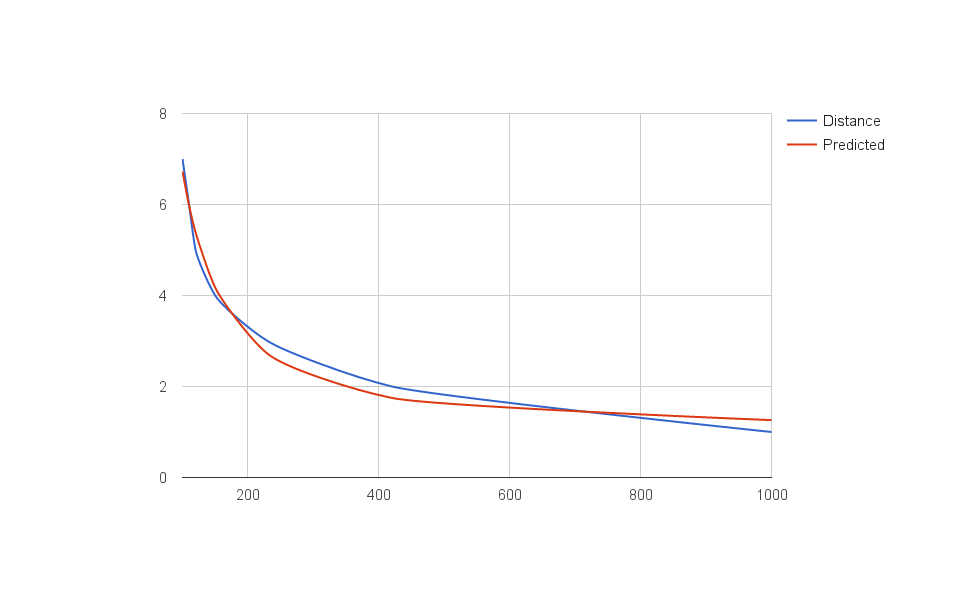
\includegraphics[width=30em]{../assets/plots/sensor-equation.png}
  \end{center}
  \begin{equation}
    S = 1.074519 + 
    \frac{9.502961}
         {(1 + \frac{\alpha}{70.42612}^{69.9039})^{0.02119919}}
  \end{equation}
  \caption{Solved equation translation betweek $S$, the distance, and $\alpha$, 
    the raw activation data of the sensor.}
\end{figure}

The reference pane transformation is performed by a ${3\times3}$ matrix, rotating and translating
onto the global reference pane.

\newpage
\subsection{mapping}

A simple map is evolved as the Robot explores it's environment. We can derive solids in the environment
from the distance sensor readings, by discarding distances above a given threshold but persisting a
PointCloud of \textit{voxels} for any readings that are closer than this threshold. These voxels (a 3D pixel)
are colorised by proximity to the robot -- bluer indicates a farther point, redder indicates closer.

\begin{figure}[H]
  \begin{center}
    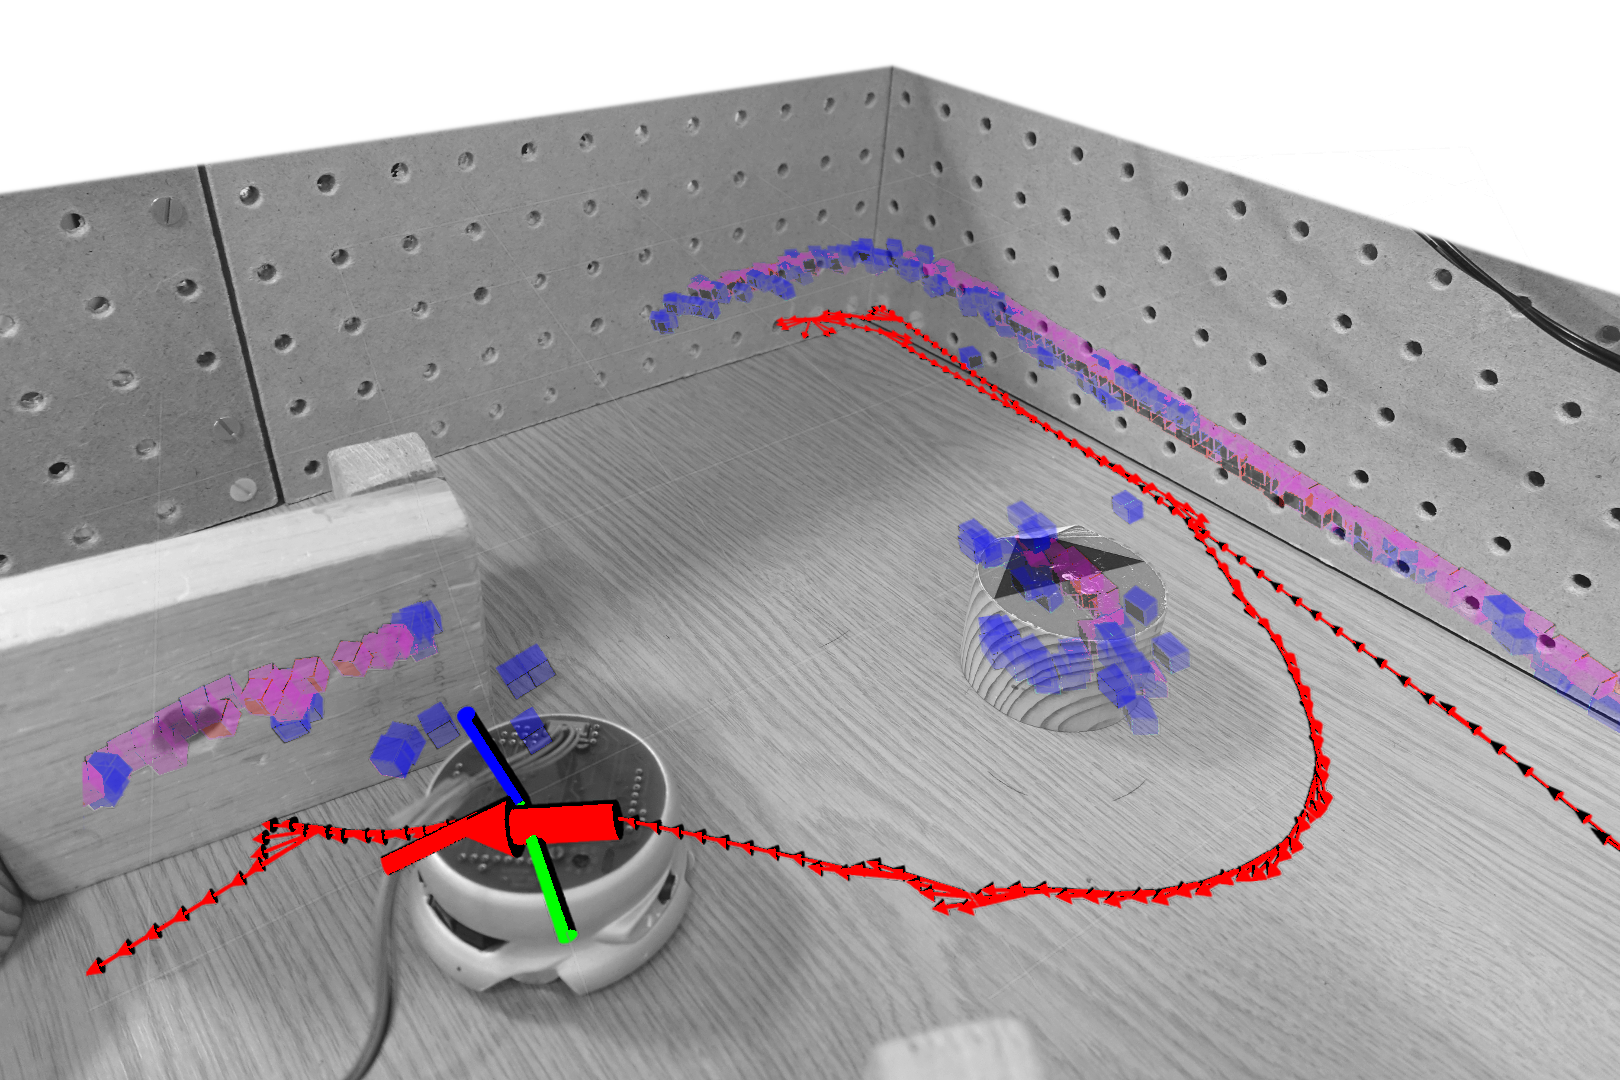
\includegraphics[width=25em]{../assets/environments/success_2_detail_merged.png}
  \end{center}
  \caption{Voxel map, Pose (red arrow), Origin and Odometry trail overlaid onto an image of the \textit{Khepera} 
  and environment taken from the same perspective. Voxels are placed at the Khepera's `eye level' of 16mm.}
\end{figure}

\begin{figure}[H]
  \begin{center}
    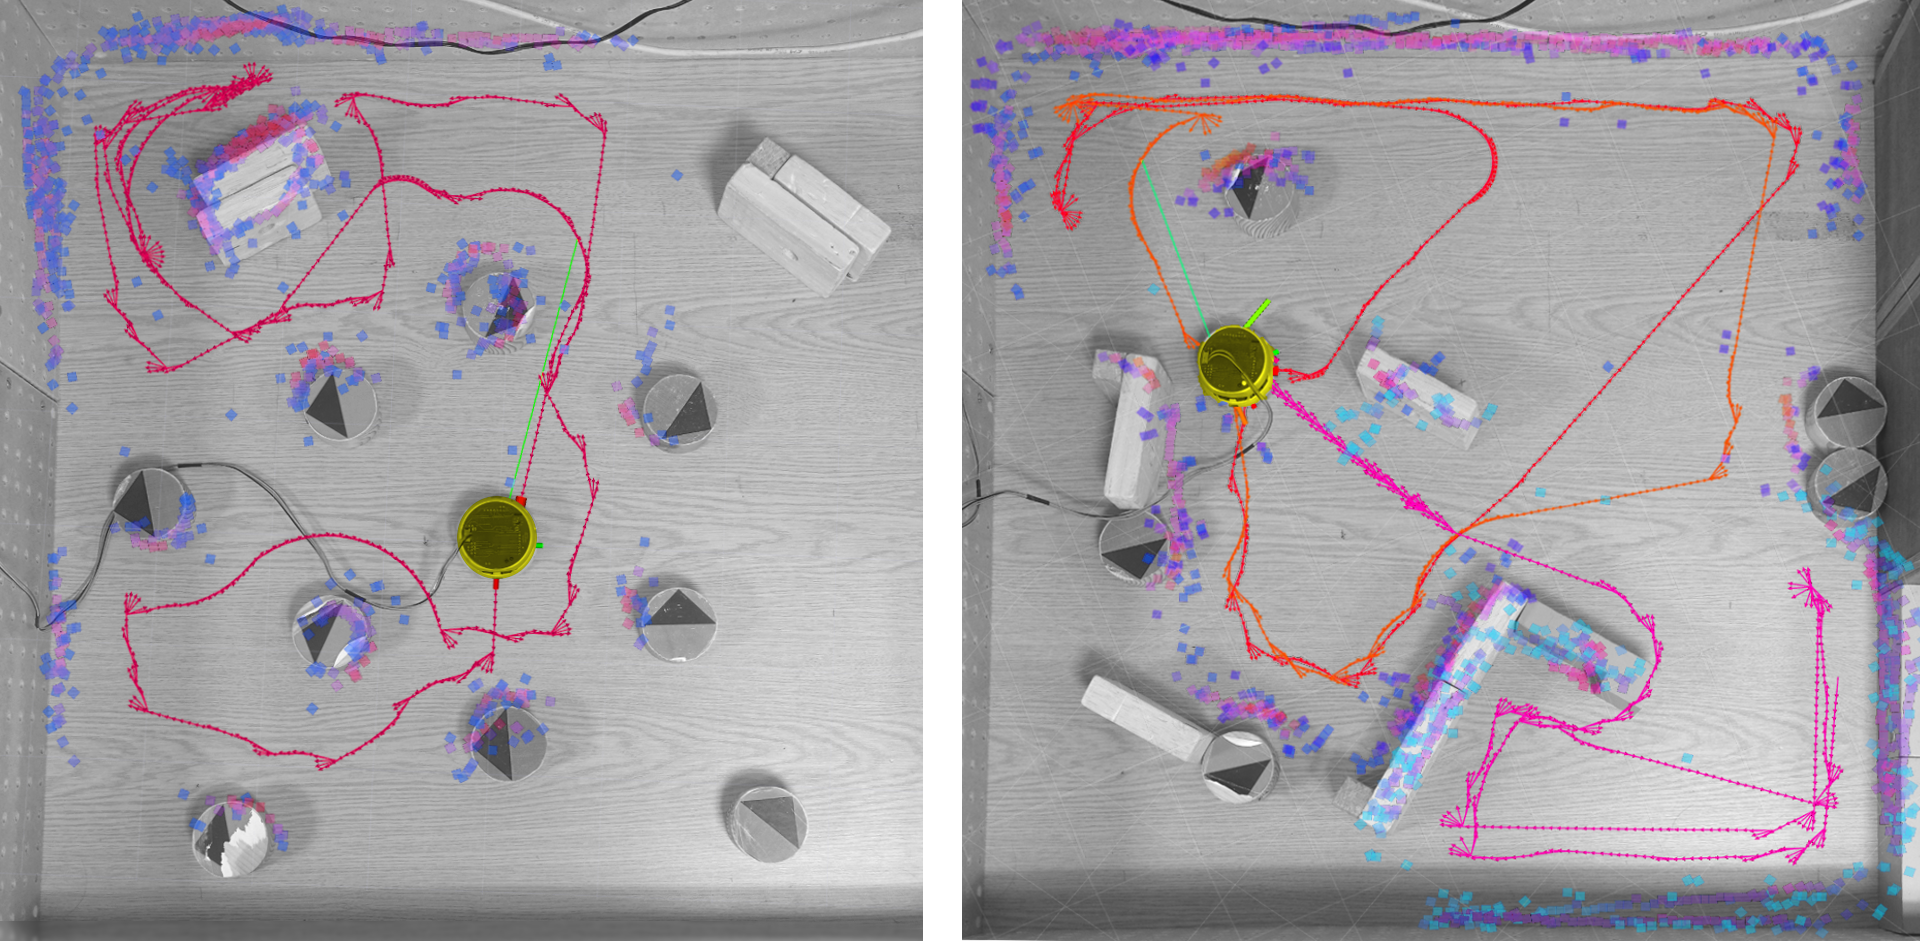
\includegraphics[width=38em]{../assets/merged_top_fig.png}
  \end{center}
  \caption{Top-down Rviz plot overlaid on a photograph of the environment, showing \textbf{left}
    a long duration (\textasciitilde1min) exploration, and \textbf{right} multiple explorations 
    and returns, where a different route was taken each time. The \textit{Khepera} 
    is highlighted in yellow at it's home location.}
\end{figure}


%       ^v^v^v^v^v^v^v^v^v^v^v^v^v^v^v^v^v^v^v^v^v^v^v^v^v^v^v^v^v^v^v^v^v^v^v^

\section{Experimental Results}
\label{Results}

In our testing, with two different and complex environments measuring roughly $1$m by $2$m the robot
successfully returned to within $10$cm of it's starting position after 30 seconds of unguided exploration
in 17/20 tests. The Robot took a different path in each excursion because it was manually guided in the 
first few seconds by the operator placing a temporary obstacle in it's way. Figure \ref{resultsfigure} 
shows the plots of these excursions separated by the two test environments. Both environments contain
sparesely populated and dense areas, and `traps' that require correct Bug behaviour to navigate.

The three failures to return to the home location were due to odometry drift -- the robot completed at a
location it believed was withing $10$cm of home but was in fact further away. One excursion had a near
algorithm failure, this eventually cleared and the robot successfully returned home. This incident
is visible in the top image depicting the first 10 trials, bottom left where there is an excess of 
voxels and odometry.

\begin{figure}[H]
  \begin{center}
    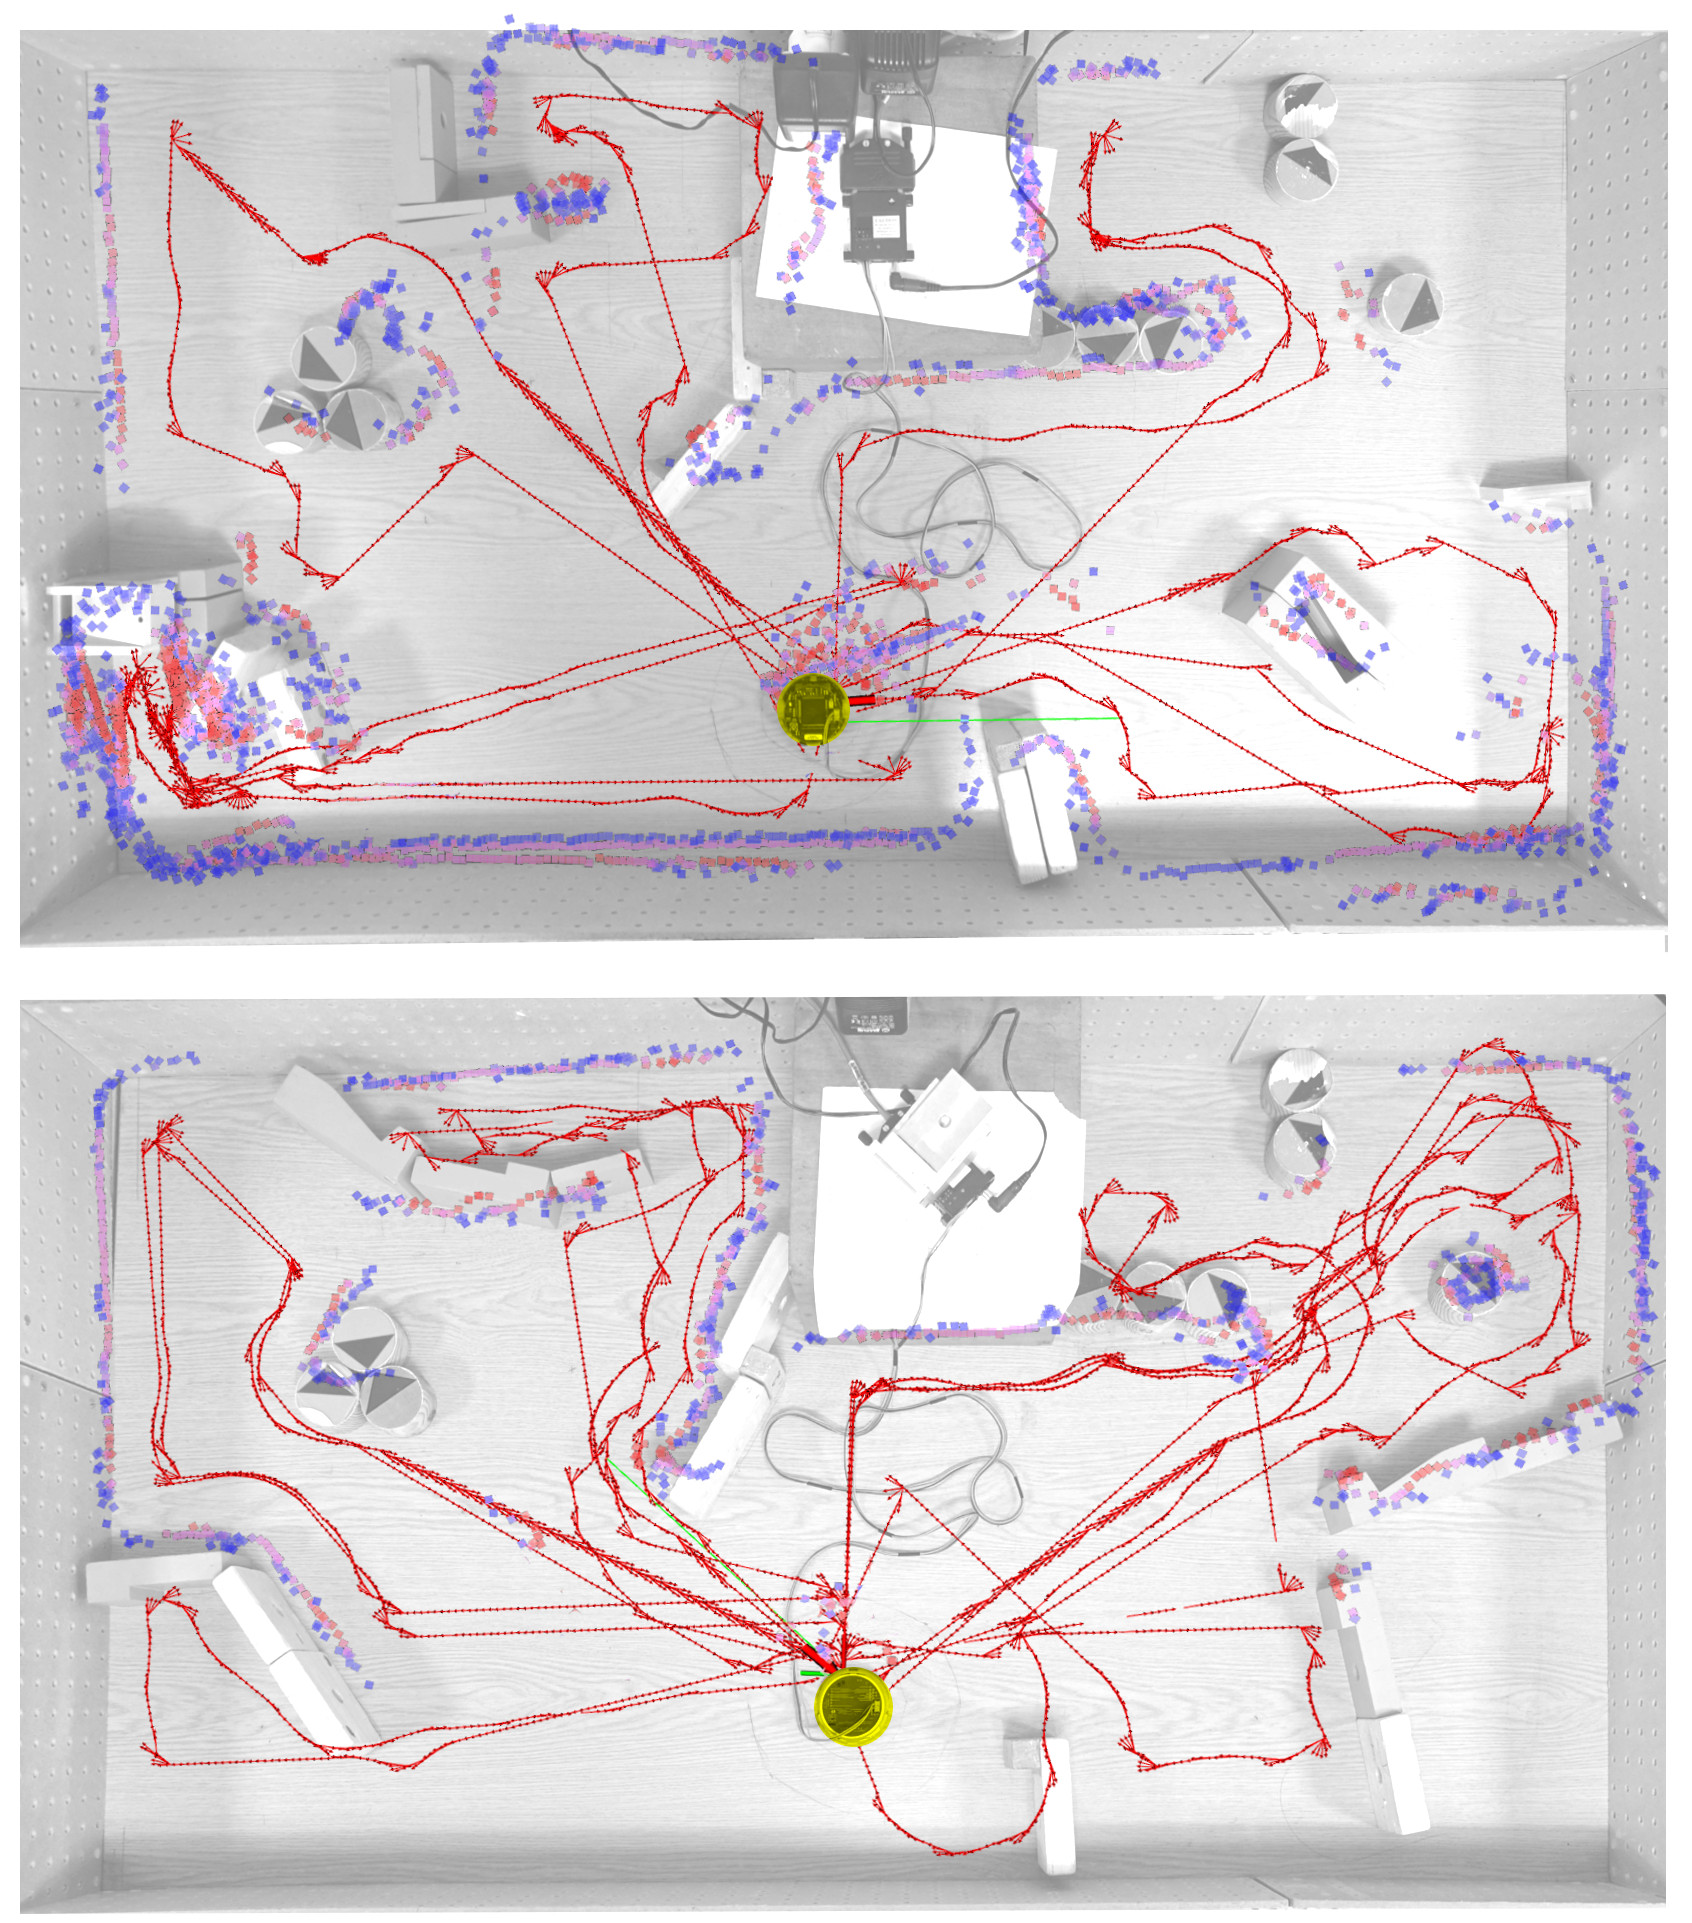
\includegraphics[width=35em]{../assets/multi_explore_figure.jpg}
  \end{center}
  \caption{\label{resultsfigure} Tracks from the two test sets overlaid on a photograph of the environment.
  \textbf{Top:} The first $10$ trials, \textbf{Bottom:} the second $10$ trials.}
\end{figure} 

%       ^v^v^v^v^v^v^v^v^v^v^v^v^v^v^v^v^v^v^v^v^v^v^v^v^v^v^v^v^v^v^v^v^v^v^v^

\newpage
\section{Discussion \& Possible Improvements}

\label{Discussion}

Various system implementation methods were researched, best ones chosen, implemented and 
tested in both sparse and dense environment for both short and long periods of time.

Odometry drift increases with time, and with the number of turns taken. However, the path that was taken
by the robot, the angles of the turns and distances were identified very accurately. Even though it worked
very well in highly dense environments the above errors were minimal in sparse environments.

The live plotting was highly effective and not only allowed us to properly test our odometry as well as 
return algorithm, but also visualize the environment in a highly comprehensible and inforamtive way. 
Moreover, it uses a separate data server, which means if the main program crashes the data is not lost,
and data can persist and be played back through Rviz later. Furthermore, we have solved a 
formula for the distance to the obstacle based on the IR values. Lastly, the current system facilitates an 
easy move towards SLAM \textit{(hint hint)}.

The subsumptious hybrid architecture that was developed between the three algorithms (as described
before) worked effectively and allowed the robot to properly switch between behaviors. The return 
algorithm's precision depends on positioning errors, so it's error is derived almost entirely from 
odometry. However, it worked with a very high sucess rate, getting stuck in only edge cases where it would 
be trapped in a very deep pocket which protruded almost towards the goal and had long walls.

Attempts to correct the algorithmic flaws were made as per above and in \textit{\S\ref{Needed Alterations}
Needed Alterations} and could yield better results if wall following is fixed to where the approach that we used would not be needed, leaving the algorithm a faithful implementation of \textit{Bug 2}.

The prime targets for improvement are our trigonometric calculations, and a supplementary localisation
technique to counteract the odometry error which is currently our limiting factor.
However, we would consider it a sucessful odometric, plotting and returning hybrid subsumptious 
mobile autonomous system\texttrademark.


%       ^v^v^v^v^v^v^v^v^v^v^v^v^v^v^v^v^v^v^v^v^v^v^v^v^v^v^v^v^v^v^v^v^v^v^v^

\newpage
\begin{thebibliography}{9}

\bibitem{principlesrobot} % The bug one
\par{Principles of Robot Motion: Theory, Algorithms, and Implementation \S2.1 `Bug Algorithms'}\\
\textit{Howie Choset}

\bibitem{Redis}
\par{Redis is an open source (BSD licensed), in-memory data structure store, used as database, cache and message broker. It supports data structures such as strings, hashes, lists, sets, sorted sets with range queries, bitmaps, hyperloglogs and geospatial indexes with radius queries.}\\
\textit{http://redis.io}

\bibitem{ROS}
\par{The Robot Operating System (ROS) is a flexible framework for writing robot software. It is a collection of tools, libraries, and conventions that aim to simplify the task of creating complex and robust robot behavior across a wide variety of robotic platforms.}\\
\textit{http://www.ros.org/}

\bibitem{runge_kutta} 
\par{Fourth order Runge - Kutta algorithm for pose estimation} \\
\textit{https://www.cs.cmu.edu/afs/cs.cmu.edu/academic/class/16311/www/s07/labs/NXTLabs/Lab\%203.html}

\bibitem{odo_used}
\par{Princeton University lecture on Autonomous Robot Navigation with odometry formulas and their deriviation from geometry and trigonometry. These formulas are devised specifically for differential drive robots} \\
\textit{https://www.cs.princeton.edu/courses/archive/fall11/cos495/COS495-Lecture5-Odometry.pdf }

\bibitem{odo_calibration} 
\par{The Technic Gear website article dealign with differential drive robot odometry calculations} \\
\textit{http://thetechnicgear.com/2014/06/howto-calibrate-differential-drive-robot/}

\bibitem{khepera_paper} 
\par{A paper on Experimental Odometry Calibration of the Mobile Robot Khepera II Based on the Least-Squares Technique from which we took inspiration on calibration and confirmation we are doing odometry in the right fashion} \\
\textit{http://ieeexplore.ieee.org/stamp/stamp.jsp?arnumber=1570321}

\bibitem{khepera_manual} 
\par{Khepera 2 user Manual containing all the fundamental information about the Khepera 2 robot, including information abotu encoders and their value meanings} \\
\textit{http://ftp.k-team.com/khepera/documentation/Kh2UserManual.pdf}

\bibitem{task1_report} 
\par{IAR 2016 Task1 Report} \\
\textit{Angus Pearson, Jevgenij Zubovskij}

\end{thebibliography}

\newpage
\begin{appendices}
\section*{Appendix}
\subsection{Code Listings}
\lstinputlisting[language=python]{../../main.py}
\lstinputlisting[language=python]{../../data.py}
\lstinputlisting[language=python]{../../comms.py}
\lstinputlisting[language=python]{../../state.py}
\lstinputlisting[language=python]{../../bug_state.py}
\lstinputlisting[language=python]{../../bug_algorithm.py}
\lstinputlisting[language=python]{../../navigation_state.py}
\lstinputlisting[language=python]{../../navigation_algorithm.py}
\lstinputlisting[language=python]{../../odometry_algorithm.py}
\lstinputlisting[language=python]{../../odometry_state.py}
\lstinputlisting[language=python]{../../constants.py}
\lstinputlisting{../../requirements.txt}
\end{appendices}


\end{document}
